\documentclass[a4paper]{article}

\usepackage{pgfplots}

\pgfplotsset{compat=1.5}

\begin{document}

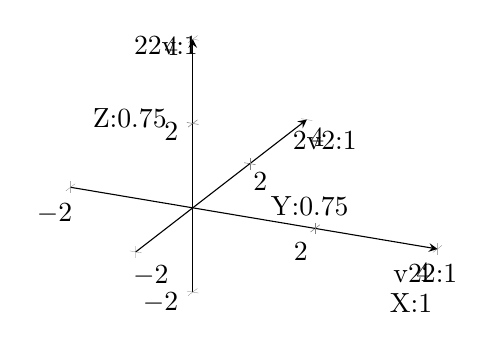
\begin{tikzpicture}
	\begin{axis}[axis lines=center,min=-2,max=4,clip=false,%disabledatascaling,
		extra description/.code={
			\node at (xticklabel cs:1) {X:1};
			\node at (yticklabel cs:0.75) {Y:0.75};
			\node at (zticklabel cs:0.75) {Z:0.75};
			{
				\pgftransformshift{\pgfplotsqpointoutsideofaxisrel{v22}{1}{10pt}}%
				\node at (0pt,0pt) {v22:1};
			}
			{
				\pgftransformshift{\pgfplotsqpointoutsideofaxisrel{2v2}{1}{10pt}}%
				\node at (0pt,0pt) {2v2:1};
			}
			{
				\pgftransformshift{\pgfplotsqpointoutsideofaxisrel{22v}{1}{10pt}}%
				\node at (0pt,0pt) {22v:1};
			}
		}
	]
	\end{axis}
\end{tikzpicture}

%\FIXIT
\end{document}

